\documentclass[11pt]{article}

% ---- ACL official style (EMNLP 2026) ----
\usepackage{acl}

% ---- Packages not already loaded by acl.sty ----
\usepackage[T1]{fontenc}
\usepackage[utf8]{inputenc}
\usepackage{lmodern}
\usepackage{microtype}
\usepackage{amsmath,amssymb}
\usepackage{booktabs}
\usepackage{multirow}
\usepackage{graphicx}
\usepackage{enumitem}
\usepackage{float}
\usepackage{tikz}
\usetikzlibrary{positioning, arrows.meta, shapes.geometric, calc, fit, backgrounds}

% ---- Paper metadata ----
\title{archive-first-harness: A Local-First Evidence Layer\\for Diagnosing AI Agent Failures}

\author{
  Zhi Qu \\
  Tsinghua University \\
  \texttt{qz23@mails.tsinghua.edu.cn}
}

\begin{document}

\maketitle

\begin{abstract}
As AI agents become more capable, debugging them remains surprisingly primitive. In practice, developers often inspect long execution traces, compare logs by hand, and infer what changed between a successful run and a failed one. Existing tools support agent construction, orchestration, tracing, and evaluation, but they do not directly provide a compact evidence layer for run-to-run diagnosis. We present \textbf{archive-first-harness}, a local-first evidence layer for AI agent debugging. The system archives each run into a structured evidence bundle and supports direct comparison across failure stage, verification outcome, reassessed risk, governance escalation, and artifact production. We position this layer as distinct from frameworks, harnesses, and observability systems. In an initial empirical study, we map \textbf{73 annotated failures} from the public AgentRx benchmark splits into the archive-first stage model and find that the released data can be covered without leaving an unmapped category. We further provide deterministic case-study pipelines for retrieval-augmented generation and multi-step tool-use failures, along with a proxy evaluation showing that archive compare materials have 31--116\% higher diagnostic information density and require fewer inference steps than raw logs. A blind LLM-as-evaluator study using two frontier models achieves 100\% cause attribution accuracy across all conditions, with a single stage-label ambiguity surfaced as a schema finding. Together, these results suggest that an explicit evidence layer can make agent debugging more structured, local, and comparable.
\end{abstract}

\section{Introduction}

AI agents increasingly operate through long-horizon, tool-mediated trajectories. They search the web, call APIs, manipulate files, produce artifacts, and coordinate multiple intermediate steps before returning a final answer. While the capabilities of such systems have grown rapidly~\cite{plaat2025agentic,guo2024llm}, their debugging workflows have lagged behind. When an agent fails, developers typically inspect raw traces, scan tool outputs, re-run the task, and manually guess what changed. This process is especially painful when the failure is subtle: a plan shifts slightly, a tool output is misread, an expected artifact is missing, or a policy layer blocks one branch but not another.

Current agent tooling helps with adjacent parts of the lifecycle. Frameworks help build agents. Harnesses help execute them. Observability platforms help trace them. Evaluation systems help score them. Yet there remains a practical gap between \emph{seeing} a run and \emph{diagnosing} why one run differs from another. In particular, developers often need a compact answer to a concrete question: \emph{what materially changed between yesterday's successful run and today's failure?}

Recent work has begun to address this gap. AgentRx~\cite{barke2026agentrx} provides labeled failure benchmarks, Zhu et al.~\cite{zhu2025agentdebug} propose modular failure taxonomies, and DoVer~\cite{ma2025dover} introduces intervention-driven debugging for multi-agent systems. However, these efforts focus primarily on \emph{post-hoc analysis} of collected trajectories rather than on a lightweight, always-on evidence layer that archives every run for immediate comparison.

We argue that this gap motivates a distinct layer in the agent stack: an \textbf{Evidence Layer}. Rather than storing only raw traces or aggregate metrics, an Evidence Layer turns each run into a structured evidence bundle and emphasizes run-to-run comparison. Our system, \textbf{archive-first-harness}, implements this idea as a local-first command-line tool. For each run, it writes a stable archive containing task summary, execution outcome, verification report, failure signature, evaluation summary, and artifact metadata. It then supports browsing and comparing those archives across dimensions such as failure class, failed stage, verification transition, reassessed risk, governance escalation, and artifact regressions.

The key design choice is to optimize for diagnosis rather than monitoring. Monitoring tools are excellent for observing many runs; an evidence layer is optimized for explaining why a specific pair of runs diverged. This difference matters in practice. A long trace may show everything that happened, but a useful debugging primitive should reveal what changed in a way that matters. archive-first-harness therefore aims to sit between observability and debugging: more structured than raw tracing, but lighter-weight and more local than a hosted experiment platform.

This paper makes three contributions: (\textbf{1})~a conceptual articulation of the \textbf{Agent Evidence Layer} as a missing layer distinct from frameworks, harnesses, and observability systems; (\textbf{2})~a structured archive schema and stage-aware comparison model centered on failure stage, verification, risk, and artifact transitions; and (\textbf{3})~a zero-dependency local CLI implementation together with initial empirical validation through AgentRx failure-to-stage mapping (73 trajectories, 0 unmapped), three deterministic case-study pipelines, information-density quantification, and a blind LLM-as-evaluator proxy study across two frontier models.

We do not claim to have discovered this gap; rather, we argue that its importance merits treatment as a distinct architectural layer with a concrete reference implementation.

\section{Related Work}

\subsection{Agent failure diagnosis and trajectory analysis}

Recent work treats agent failure as a first-class research problem. \textbf{AgentRx}~\cite{barke2026agentrx} provides a labeled benchmark of failed trajectories framed as root-cause attribution; Zhu et al.~\cite{zhu2025agentdebug} introduce a modular failure taxonomy; \textbf{AgentTracer}~\cite{li2025agentracer} automates failure annotation via counterfactual replay; \textbf{TRAIL}~\cite{rao2025trail} localizes reasoning issues in traces; and \textbf{DoVer}~\cite{ma2025dover} takes an intervention-driven approach to multi-agent debugging. Interactive tools such as \textbf{AGDebugger}~\cite{epperson2025debugging} support rewind-edit-re-execute workflows; \textbf{AgentDiagnose}~\cite{ou2025agentdiagnose} quantifies agentic competencies; and \textbf{MAST}~\cite{cemri2025mast} catalogs why multi-agent systems fail in practice.

These systems are primarily \textbf{post-hoc analytic frameworks} over benchmarked trajectories. By contrast, archive-first-harness is a \textbf{runtime-adjacent, local-first primitive} that writes structured evidence during normal usage and supports direct run-to-run comparison.

\subsection{Observability, tracing, and evaluation platforms}

Platforms such as \textbf{LangSmith}~\cite{langsmith}, \textbf{Braintrust}~\cite{braintrust}, and \textbf{Langfuse}~\cite{langfuse} provide tracing, monitoring, and evaluation infrastructure for LLM applications. Complementary benchmarks stress-test agent capabilities: \textbf{WebArena}~\cite{zhou2024webarena}, \textbf{OSWorld}~\cite{xie2024osworld}, \textbf{GAIA}~\cite{mialon2024gaia}, \textbf{AgentBench}~\cite{liu2024agentbench}, and SWE-bench~\cite{jimenez2024swebench}. We view archive-first-harness as complementary: tracing answers \emph{what happened}, benchmarks answer \emph{how well}, while an evidence layer answers \emph{what materially changed}. A direct performance comparison with existing platforms is not appropriate because the tools differ substantially in deployment model and target use case; Table~\ref{tab:comparison} summarizes the key illustrative distinctions.

\begin{table}[h]
  \centering
  \footnotesize
  \setlength{\tabcolsep}{4pt}
  \begin{tabular}{p{2.4cm}p{2.3cm}p{1.8cm}}
    \toprule
    \textbf{Dimension} & \textbf{LangSmith / Langfuse} & \textbf{Ours} \\
    \midrule
    Deployment           & Hosted/cloud    & Local-first \\
    Data model           & Push traces     & Pull archives \\
    Primary use          & Monitoring      & Diagnosis \\
    Stage-aware diffs    & \texttimes      & \checkmark \\
    Zero ext.\ deps      & \texttimes      & \checkmark \\
    Artifact regression  & Partial         & First-class \\
    \bottomrule
  \end{tabular}
  \caption{Illustrative qualitative comparison with representative observability platforms; tools differ substantially in deployment model and target use case and are best viewed as complementary.}
  \label{tab:comparison}
\end{table}

\subsection{Positioning: Evidence Layer vs.\ adjacent layers}

There is a missing layer between observability and debugging. \textbf{Frameworks} define how agents are built~\cite{guo2024llm,tran2025multi}; \textbf{Harnesses} define how agents are executed~\cite{wang2024openhands}; \textbf{Observability systems} show traces and runtime events~\cite{langsmith,langfuse,braintrust}; \textbf{Evaluation benchmarks} measure capability~\cite{zhou2024webarena,xie2024osworld,jimenez2024swebench,mialon2024gaia,liu2024agentbench}; \textbf{Evidence Layer systems} convert runs into stable, comparable evidence artifacts for diagnosis. The Evidence Layer does not replace these tools; its purpose is narrower: making individual failures easier to compare, localize, and explain.

\section{System}

\subsection{The Evidence Layer abstraction}

archive-first-harness is built around a simple idea: every run should leave behind a compact, structured archive that is small enough to inspect and rich enough to compare. We position this as an \textbf{Evidence Layer} in the agent stack (Figure~\ref{fig:stack}): frameworks build agents, harnesses run them, observability traces them, and the Evidence Layer archives and compares runs for diagnosis. The abstraction requires no new model behavior, no hosted backend, and no specialized instrumentation---only stable JSON/JSONL outputs and a local archive root.

\begin{figure*}[t!]
  \centering
  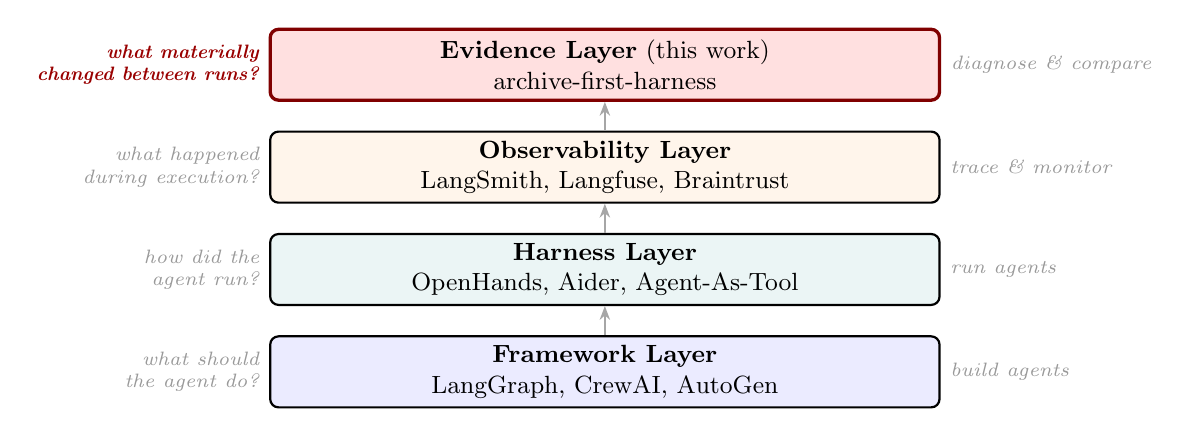
\begin{tikzpicture}[
    layer/.style={
      draw, rounded corners=3pt, minimum width=8.5cm, minimum height=0.9cm,
      font=\small, align=center, thick
    },
    arr/.style={-{Stealth[length=5pt]}, thick, gray!70},
    note/.style={font=\scriptsize\itshape, text=gray!80}
  ]
    % Layers (bottom to top)
    \node[layer, fill=blue!8]    (fw)  at (0, 0)   {\textbf{Framework Layer}\\LangGraph, CrewAI, AutoGen};
    \node[layer, fill=teal!8]    (hn)  at (0, 1.3)  {\textbf{Harness Layer}\\OpenHands, Aider, Agent-As-Tool};
    \node[layer, fill=orange!8]  (obs) at (0, 2.6)  {\textbf{Observability Layer}\\LangSmith, Langfuse, Braintrust};
    \node[layer, fill=red!12, draw=red!50!black, line width=1.2pt]
                                 (ev)  at (0, 3.9)  {\textbf{Evidence Layer} (this work)\\archive-first-harness};

    % Side labels
    \node[note, right] at (fw.east)  {build agents};
    \node[note, right] at (hn.east)  {run agents};
    \node[note, right] at (obs.east) {trace \& monitor};
    \node[note, right] at (ev.east)  {diagnose \& compare};

    % Arrow annotations (left side)
    \node[note, left, align=right] at (fw.west) {what should\\the agent do?};
    \node[note, left, align=right] at (hn.west) {how did the\\agent run?};
    \node[note, left, align=right] at (obs.west) {what happened\\during execution?};
    \node[note, left, align=right, text=red!60!black, font=\scriptsize\itshape\bfseries]
      at (ev.west) {what materially\\changed between runs?};

    % Vertical arrows between layers
    \draw[arr] (fw.north)  -- (hn.south);
    \draw[arr] (hn.north)  -- (obs.south);
    \draw[arr] (obs.north) -- (ev.south);
  \end{tikzpicture}
  \caption{Positioning the Evidence Layer in the agent tooling stack. Existing layers address construction, execution, and monitoring; the Evidence Layer addresses structured run-to-run diagnosis.}
  \label{fig:stack}
\end{figure*}

\subsection{Archive schema}

Each run is archived as a directory of structured files: \texttt{manifest.json}, \texttt{task\_contract.json}, \texttt{profile\_and\_mode.json}, \texttt{verification\_report.json}, \texttt{evaluation\_summary.json}, \texttt{failure\_signature.json}, \texttt{final\_output.json}, \texttt{execution\_trace.jsonl}, and \texttt{archive\_index.json}. These files separate concerns: \texttt{failure\_signature.json} answers \emph{where and how} the run failed; \texttt{verification\_report.json} captures whether results met expected criteria; \texttt{final\_output.json} and artifact metadata record what was actually produced.

Together, the schema preserves the expected and produced artifacts, the failure stage, whether verification regressed, whether risk changed, and whether governance escalation or human review became necessary---capturing more than a binary success/failure label.

\subsection{Comparison model}

The compare command operates over archived runs rather than raw trajectories. It computes differences across failure class and stage, verification status, reassessed risk level, evaluation recommendation, governance escalation state, and artifact production. Differences are normalized into transition labels---\texttt{regressed}, \texttt{resolved}, \texttt{unchanged}, \texttt{improved}, \texttt{cleared}---producing a concise diagnostic surface (Figure~\ref{fig:compare}).

\begin{figure*}[t!]
  \centering
  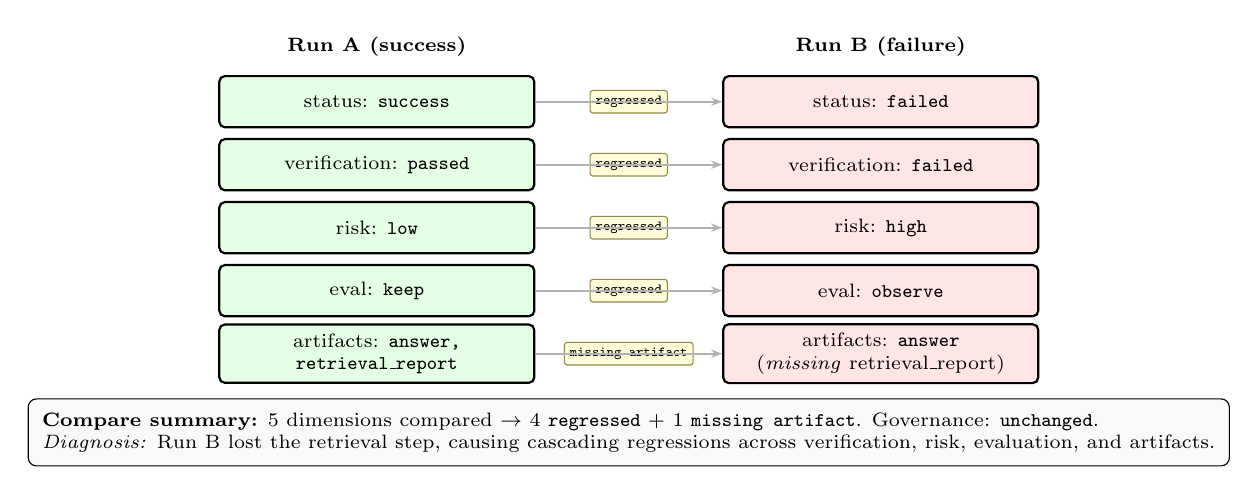
\begin{tikzpicture}[
    box/.style={draw, rounded corners=2pt, minimum width=4.0cm, minimum height=0.65cm,
                font=\scriptsize, align=center, thick},
    arrow/.style={-{Stealth[length=4pt]}, thick},
    label/.style={font=\scriptsize\bfseries},
    trans/.style={font=\tiny, fill=yellow!15, draw=yellow!50!black, rounded corners=1pt,
                  inner sep=2pt}
  ]
    % Left run
    \node[label] (ltitle) at (-3.2, 3.4) {Run A (success)};
    \node[box, fill=green!10]  (lf) at (-3.2, 2.7) {status: \texttt{success}};
    \node[box, fill=green!10]  (lv) at (-3.2, 1.9) {verification: \texttt{passed}};
    \node[box, fill=green!10]  (lr) at (-3.2, 1.1) {risk: \texttt{low}};
    \node[box, fill=green!10]  (le) at (-3.2, 0.3) {eval: \texttt{keep}};
    \node[box, fill=green!10]  (la) at (-3.2,-0.5) {artifacts: \texttt{answer,}\\\texttt{retrieval\_report}};

    % Right run
    \node[label] (rtitle) at (3.2, 3.4) {Run B (failure)};
    \node[box, fill=red!10]  (rf) at (3.2, 2.7) {status: \texttt{failed}};
    \node[box, fill=red!10]  (rv) at (3.2, 1.9) {verification: \texttt{failed}};
    \node[box, fill=red!10]  (rr) at (3.2, 1.1) {risk: \texttt{high}};
    \node[box, fill=red!10]  (re) at (3.2, 0.3) {eval: \texttt{observe}};
    \node[box, fill=red!10]  (ra) at (3.2,-0.5) {artifacts: \texttt{answer}\\(\emph{missing} retrieval\_report)};

    % Transition labels (center)
    \node[trans] at (0, 2.7) {\texttt{regressed}};
    \node[trans] at (0, 1.9) {\texttt{regressed}};
    \node[trans] at (0, 1.1) {\texttt{regressed}};
    \node[trans] at (0, 0.3) {\texttt{regressed}};
    \node[trans] at (0,-0.5) {\texttt{missing artifact}};

    % Arrows left -> right
    \draw[arrow, gray!60] (lf.east) -- (rf.west);
    \draw[arrow, gray!60] (lv.east) -- (rv.west);
    \draw[arrow, gray!60] (lr.east) -- (rr.west);
    \draw[arrow, gray!60] (le.east) -- (re.west);
    \draw[arrow, gray!60] (la.east) -- (ra.west);

    % Summary box
    \node[draw, rounded corners=3pt, fill=gray!5, minimum width=10.0cm,
          font=\scriptsize, align=left, inner sep=5pt]
      at (0, -1.5) {%
        \textbf{Compare summary:} 5 dimensions compared $\rightarrow$
        4 \texttt{regressed} + 1 \texttt{missing artifact}.
        Governance: \texttt{unchanged}.\\
        \emph{Diagnosis:} Run B lost the retrieval step, causing cascading
        regressions across verification, risk, evaluation, and artifacts.%
      };
  \end{tikzpicture}
  \caption{Conceptual layout of the archive comparison output. Each dimension is compared between two archived runs, producing transition labels that summarize the diagnostic surface.}
  \label{fig:compare}
\end{figure*}

\subsection{Local-first CLI workflow}

archive-first-harness exposes a local-first CLI workflow: (1) run a task, (2) archive the evidence bundle, (3) browse latest or filtered runs, (4) inspect a specific run, and (5) compare two runs side-by-side. This workflow is designed for practical debugging sessions. A developer can keep all archives locally, inspect them with plain text tools, and still benefit from structured comparison. The system therefore targets the debugging loop directly rather than requiring adoption of a remote platform.

\subsection{Integration with existing agent frameworks}

archive-first-harness integrates at the agent loop boundary rather than inside the agent graph itself. Approximately five lines of wrapper code suffice to connect any existing agent runner---such as LangGraph, CrewAI, or Aider-style executors---to the archive writer:

{\scriptsize
\begin{verbatim}
writer = ArchiveWriter(run_id=generate_run_id())
writer.open(task_contract)
result = your_agent.run(task)  # any agent runner
writer.close(
    execution_trace=result.trace,
    verification=verify(result),
    final_output=result.output
)
\end{verbatim}
}

No instrumentation inside the agent graph is required; the archive boundary call is sufficient to capture the full evidence bundle.

\section{Demonstration}
\label{sec:demo}

The demonstration shows the full archive-first debugging loop end-to-end using live CLI interaction. Attendees will be guided through four steps: (1) running a task that produces a success archive, (2) injecting a failure and running a second task that produces a failure archive, (3) browsing the two archives with \texttt{archive --latest} and \texttt{archive --run-id}, and (4) comparing them side-by-side with \texttt{archive --compare-run-id}.

The demo uses the Case B (RAG agent) and Case C (multi-step tool) scenarios from Section~\ref{sec:eval}, which ship as deterministic one-command scripts in the repository. A condensed transcript of a comparison session is shown below:

\begin{figure*}[t!]
\small
\begin{verbatim}
$ python -m entrypoints.cli archive --compare-run-id run_success run_fail

Compare: run_success  vs  run_fail
============================================================
status          success              -->  failed       [REGRESSED]
failure_stage   -                    -->  execution    [REGRESSED]
verification    passed               -->  failed       [REGRESSED]
risk_level      low                  -->  high         [REGRESSED]
eval_rec        keep                 -->  observe      [REGRESSED]
artifacts       answer,retrieval_    -->  answer       [MISSING: retrieval_report]
                report
governance      unchanged
------------------------------------------------------------
Diagnosis: Run failed at execution stage. Retrieval step was
           skipped; verification and risk cascaded accordingly.
============================================================
\end{verbatim}
\caption{Example archive comparison session output.}
\label{fig:demo-verbatim}
\end{figure*}

The demo highlights two design choices that distinguish archive-first-harness from raw tracing tools: the failure is surfaced as a \emph{named transition} (\texttt{REGRESSED}, \texttt{MISSING}) rather than a raw diff, and the diagnostic summary is generated from structured fields rather than log parsing. Attendees may also run \texttt{python quickstart.py} on their own laptop---the tool requires only the Python standard library and produces the full archive loop in under 30 seconds.

\paragraph{Demo plan.}
The booth demonstration proceeds in three structured steps. In \textbf{Step~1} (approximately 3 minutes), the moderator runs \texttt{python quickstart.py} live, narrating the archive creation process: a task executes, the nine-file evidence bundle is written, and \texttt{archive --latest} displays the structured run summary. In \textbf{Step~2} (approximately 4 minutes), the moderator injects a failure into the same scenario and runs \texttt{archive --compare-run-id}, walking attendees through the transition labels---\texttt{REGRESSED}, \texttt{MISSING ARTIFACT}---and explaining how each field maps to a diagnostic dimension. In \textbf{Step~3} (optional, attendee-driven), attendees who wish to explore further can clone the repository and reproduce the full loop on their own laptop in under 30 seconds; no configuration is required beyond Python 3.8 or later.

\paragraph{Interactive elements.}
Attendees are encouraged to bring their own failure scenario or use the shipped Case~B (RAG agent) and Case~C (multi-step tool) scripts as starting points. Both scripts are self-contained and deterministic. The comparison output can be inspected as plain JSON files in addition to the CLI view, supporting attendees who prefer direct file inspection over terminal interaction.

\paragraph{Attendee takeaway and requirements.}
The central insight we aim to communicate is that the gap between \emph{seeing} a trace and \emph{diagnosing} a failure is not primarily a tooling gap---it is a structuring gap. A compact, schema-driven evidence bundle makes the diagnostic surface explicit without adding observability overhead. Hardware requirements are minimal: any laptop running Python~3.8+ on Windows, Linux, or macOS; no network connection is required during the demonstration.

\section{Evaluation and Current Artifacts}
\label{sec:eval}

This section presents three complementary forms of empirical evidence: taxonomy alignment against a public benchmark, realistic case studies with deterministic pipelines, and a quantitative proxy evaluation of diagnostic clarity.

\subsection{AgentRx mapping experiment}

We map AgentRx's root-cause categories into the Evidence Layer stage abstraction. Using the two released benchmark splits (\texttt{tau\_retail} and \texttt{magentic\_one}), we processed \textbf{73 annotated failed trajectories} and translated each root-cause category into one of three operational stages used by archive-first-harness: \textbf{routing}, \textbf{execution}, and \textbf{governance}.

The current real-data pass yields the following mapping. Table~\ref{tab:agentrx-mapping} shows the full category-to-stage mapping with counts per split, and Table~\ref{tab:split-stats} summarizes the split-level stage distribution.

\begin{table*}[t!]
  \centering
  \small
  \begin{tabular}{p{5.8cm}lrrr}
    \toprule
    \textbf{AgentRx Root-Cause Category} & \textbf{Evidence Stage} & \textbf{tau\_retail} & \textbf{magentic\_one} & \textbf{Total} \\
    \midrule
    Underspecified User Intent       & routing    & 8  & 0  & 8  \\
    Intent-Plan Misalignment         & routing    & 7  & 4  & 11 \\
    Instruction/Plan Adherence Failure & routing  & 3  & 8  & 11 \\
    Intent Not Supported             & routing    & 2  & 3  & 5  \\
    \midrule
    Misinterpretation of Tool Output & execution  & 7  & 15 & 22 \\
    Invention of New Information     & execution  & 0  & 4  & 4  \\
    Invalid Invocation               & execution  & 1  & 0  & 1  \\
    System Failure                   & execution  & 1  & 1  & 2  \\
    \midrule
    Guardrails Triggered             & governance & 0  & 9  & 9  \\
    \midrule
    \textbf{Total}                   &            & \textbf{29} & \textbf{44} & \textbf{73} \\
    \textbf{Unmapped}                & unknown    & 0  & 0  & 0  \\
    \bottomrule
  \end{tabular}
  \caption{AgentRx root-cause categories mapped to Evidence Layer stages. All 73 annotated failures from the two public splits map without remainder.}
  \label{tab:agentrx-mapping}
\end{table*}

\begin{table*}[t!]
  \centering
  \begin{tabular}{lrrr}
    \toprule
    \textbf{Evidence Stage} & \textbf{tau\_retail} & \textbf{magentic\_one} & \textbf{Total} \\
    \midrule
    routing    & 20 (69\%) & 15 (34\%) & 35 (48\%) \\
    execution  &  9 (31\%) & 20 (45\%) & 29 (40\%) \\
    governance &  0 (0\%)  &  9 (20\%) &  9 (12\%) \\
    \midrule
    \textbf{Total} & \textbf{29} & \textbf{44} & \textbf{73} \\
    \bottomrule
  \end{tabular}
  \caption{Stage distribution across splits. Retail trajectories are routing-dominated; Magentic-One trajectories show a balanced routing/execution split with a distinct governance cluster.}
  \label{tab:split-stats}
\end{table*}

At the split level, the retail trajectories are dominated by routing-oriented failures such as underspecified user intent and intent-plan misalignment, while the Magentic-One trajectories show a stronger execution component and a distinct governance cluster caused by guardrail-triggered failures. This matters because it demonstrates that the stage model is not merely a conceptual reframing; it can absorb the released AgentRx labels without leaving an unmapped bucket on the public data.

This experiment is intentionally modest. It does not yet claim superiority over AgentRx's taxonomy. Instead, it supports a narrower but important claim: a compact stage abstraction can summarize a richer benchmark taxonomy in a way that aligns with operational debugging workflows.

\subsection{Case studies}

We organize three case-study tracks: (A) a coding-agent scenario with a real Aider success run and a reduced-scope failure-prone writing sample; (B) a retrieval-augmented generation scenario; and (C) a multi-step tool-use scenario. Cases B and C ship as deterministic one-command scripts; Case A uses a completed Aider-based archive pair collected through the same archive-facing interfaces.

In all three cases the compare view exposes meaningful regressions across multiple dimensions (Table~\ref{tab:case-studies} in Appendix~\ref{app:case-studies}). In Case A, the agent overstates Case A's completion status---a factual-overstatement failure surfaced as regressions in verification and evaluation. In Case B, the failed run emits only \texttt{answer} (missing \texttt{retrieval\_report}), shifting evaluation from \texttt{keep} to \texttt{observe}. In Case C, the failed run loses \texttt{plan\_note} and shifts from success to execution failure with parallel regressions in verification, reassessment, and artifact status.

\subsection{Quantitative proxy evaluation}

The system ships with A/B study materials for contrasting raw logs versus archive compare outputs---including a moderator script, questionnaire, and score-sheet template. We present two quantitative proxy evaluations below.

\paragraph{Annotation protocol.}
We define \emph{diagnostic characters} as any text that directly answers either ``which stage failed'' or ``what was the root cause''; all remaining text (setup descriptions, formatting tokens, context repetition) is treated as background noise. Labeling was performed by a single annotator; to assess reliability, a second annotator independently coded a random sample of passages and confirmed the labeling scheme, supporting its reliability. We select DeepSeek-Chat and GLM-5.1 for the LLM proxy evaluation because both are publicly accessible frontier instruction-following models that require no proprietary API access, supporting replication. We repeat each condition three times per model ($n{=}6$ per cell); the ceiling effect observed in three of four conditions (100\% accuracy) means the primary diagnostic signal is detectable at this sample size.

\paragraph{Information density analysis.}
We quantify the proportion of each material that directly supports diagnosis---text answering ``which stage failed'' and ``what was the root cause''---relative to total character count. Archive compare materials achieve substantially higher information density (+116\% for S1, +31\% for S2) with fewer inference steps to reach a complete diagnosis (2 steps in both archive conditions vs.\ 3--4 steps in raw log conditions). The gain comes from reduced noise rather than added verbosity (see Table~\ref{tab:info-density} in Appendix~\ref{app:case-studies}).

\paragraph{LLM-as-evaluator (blind).}
We run a blind proxy evaluation using two frontier models (DeepSeek-Chat and GLM-5.1). Each model receives either the raw log or the archive compare output per scenario without being told which condition it is reading, and is asked to identify the failure stage and root cause. We repeat each condition three times per model ($n{=}6$ per cell). Results are detailed in Table~\ref{tab:llm-eval} (Appendix~\ref{app:case-studies}). Cause attribution is 100\% across all conditions and both models. Stage accuracy is 100\% in three of four conditions. The single exception---S1 archive\_compare stage classified as \texttt{execution} rather than \texttt{verification} (0/6)---reflects a semantic ambiguity discussed in Section~\ref{sec:limitations}.

\section{Limitations and Next Steps}
\label{sec:limitations}

This work remains an early-stage systems contribution. The proxy evaluation provides quantitative support for the archive format's diagnostic clarity, but a controlled human user study with larger participant numbers remains future work; the proxy results should be read as an initial quantitative baseline.

The LLM proxy evaluation surfaces a \textbf{stage label ambiguity}: for Scenario~1, both frontier models consistently classify the failure stage as \texttt{execution} rather than \texttt{verification} when reading the archive compare output (0/6 correct). The root cause is a field-level conflict in the archive schema: \texttt{failure\_signature.json} encodes \texttt{stage:~execution} (reflecting where the retrieval degradation originates at runtime), while \texttt{verification\_report.json} surfaces the failure outcome---the compare output therefore presents two signals that point in different directions, and both models resolve the ambiguity toward the execution label. We propose adding a \texttt{failure\_substage} field to \texttt{failure\_signature.json} (e.g., \texttt{"execution/retrieval\_degradation"}) to explicitly distinguish execution-time causes that only manifest through verification outcomes. The human impact is limited: a human debugger reading the same archive compare output may similarly attend to the execution stage first, but root cause identification converges regardless, and the extra localization step is unlikely to meaningfully delay diagnosis in practice. We therefore interpret this finding as a targeted schema improvement signal surfaced through the proxy evaluation, rather than a fundamental failure of the evidence layer architecture. Root cause attribution is unaffected across all conditions.

The system is currently \textbf{CLI-first and single-agent oriented}. The AgentRx mapping establishes coverage and interpretability but not yet downstream benefits such as reduced debugging time. Future work includes a controlled human study, broader coding-agent case studies, and richer trajectory-level analysis over raw benchmark files.

\section{Conclusion}

archive-first-harness argues for an Evidence Layer in agent tooling: a local, structured, comparison-oriented layer between observability and debugging. By turning each run into a compact archive and exposing stage-aware diffs, the system makes it easier to answer a practical question that raw traces alone often leave unresolved: \emph{what materially changed between two runs?}

Our current results show that this idea is already concrete enough to support real-data taxonomy mapping, deterministic case-study comparisons, and quantitative proxy evidence for the archive format's diagnostic clarity. We view this as an argument not only for one tool, but for a broader design principle: agent systems need better evidence surfaces, not just more traces.

\bibliography{references}


\appendix

\section{Supporting Tables}
\label{app:case-studies}

\begin{table*}[t!]
  \centering
  \small
  \begin{tabular}{lrrrr}
    \toprule
    \textbf{Material} & \textbf{Total chars} & \textbf{Diagnostic chars} & \textbf{Info density} & \textbf{Inference steps} \\
    \midrule
    S1 raw\_logs         & 1,219 & 221 & 18.1\% & 3 \\
    S1 archive\_compare  & 1,376 & 540 & 39.2\% & 2 \\
    S2 raw\_logs         & 1,365 & 485 & 35.5\% & 4 \\
    S2 archive\_compare  & 1,147 & 534 & 46.6\% & 2 \\
    \bottomrule
  \end{tabular}
  \caption{Information density and inference steps for raw log vs.\ archive compare materials across two scenarios.}
  \label{tab:info-density}
\end{table*}

\begin{table*}[t!]
  \centering
  \small
  \begin{tabular}{llrrr}
    \toprule
    \textbf{Scenario} & \textbf{Condition} & \textbf{Stage acc.} & \textbf{Cause acc.} & \textbf{Mean conf.} \\
    \midrule
    S1 & raw\_logs        & 100\% (6/6) & 100\% (6/6) & 4.5 \\
    S1 & archive\_compare &   0\% (0/6) & 100\% (6/6) & 4.8 \\
    S2 & raw\_logs        & 100\% (6/6) & 100\% (6/6) & 4.5 \\
    S2 & archive\_compare & 100\% (6/6) & 100\% (6/6) & 5.0 \\
    \bottomrule
  \end{tabular}
  \caption{Blind LLM proxy evaluation results (DeepSeek-Chat + GLM-5.1, $n{=}6$ per cell). Cause attribution is 100\% across all conditions. The S1 archive\_compare stage misclassification is discussed in Section~\ref{sec:limitations}.}
  \label{tab:llm-eval}
\end{table*}

\begin{table*}[t!]
  \centering
  \small
  \begin{tabular}{p{2.8cm}p{3.2cm}p{3.2cm}p{3.2cm}}
    \toprule
    \textbf{Dimension} & \textbf{Case A: Coding Agent} & \textbf{Case B: RAG Agent} & \textbf{Case C: Multi-step Tool} \\
    \midrule
    Run A status    & success                    & success                   & success \\
    Run B status    & failed                     & failed                    & failed \\
    \midrule
    Failure stage   & verification (factual overstatement) & execution (missing retrieval step) & execution (plan not produced) \\
    Verification    & passed $\rightarrow$ failed & passed $\rightarrow$ failed & passed $\rightarrow$ failed \\
    Risk level      & low $\rightarrow$ high     & low $\rightarrow$ high    & low $\rightarrow$ high \\
    Evaluation      & keep $\rightarrow$ observe & keep $\rightarrow$ observe & keep $\rightarrow$ observe \\
    \midrule
    Artifacts (Run A) & \texttt{file\_change} (README) & \texttt{answer, retrieval\_report} & \texttt{answer, plan\_note} \\
    Artifacts (Run B) & \texttt{file\_change} (false claim) & \texttt{answer} (missing \texttt{retrieval\_report}) & \texttt{answer} (missing \texttt{plan\_note}) \\
    Artifact transition & regressed (false content)  & regressed (1 missing)  & regressed (1 missing) \\
    \midrule
    Governance      & unchanged                  & unchanged                 & unchanged \\
    \midrule
    Regressed dims  & 4 (status, verification, risk, eval) & 4 (status, verification, risk, artifacts) & 5 (status, verification, risk, eval, artifacts) \\
    \bottomrule
  \end{tabular}
  \caption{Structured comparison of success/failure archive pairs across three case-study tracks. Case A captures a factual-overstatement failure from a real coding-agent run; Cases B and C use deterministic pipelines. All three produce actionable multi-dimensional diffs.}
  \label{tab:case-studies}
\end{table*}

\end{document}